\section{Designkonzept}

% Klassenzimmer --> Flugschule um weiteren Komponenten sinnvoll einzufügen
%--> erstellung eines händischen drahtmodells -->
% --> Definition der einzelnen Komponenten --> Maße definieren
% --> Visio Zeichnung 
% --> Interaktionen definieren
% Flugsimulator als erweiterung

%//TODO Mention Phong from Flightsimulator

\subsection{Klassenzimmer}
Als grundlegende Idee wurde zunächst ein Vorlesungssaal vorgeschlagen.
Um weitere Komponenten aus den Anforderungen an diese Arbeit sinnvoll umzusetzen,
wurde die grundlegende Idee überdacht und neu definiert als Klassenzimmer einer Flugschule.
\newparagraph
Um eine erste Vorstellung des Klassenzimmers zu bekommen wurde zunächst eine händische Zeichnung angefertigt.
Diese ist in der Abbildung \ref{fig:KlassenzimmerSkizze} dargestellt.
\begin{figure}[H]
  \centering
  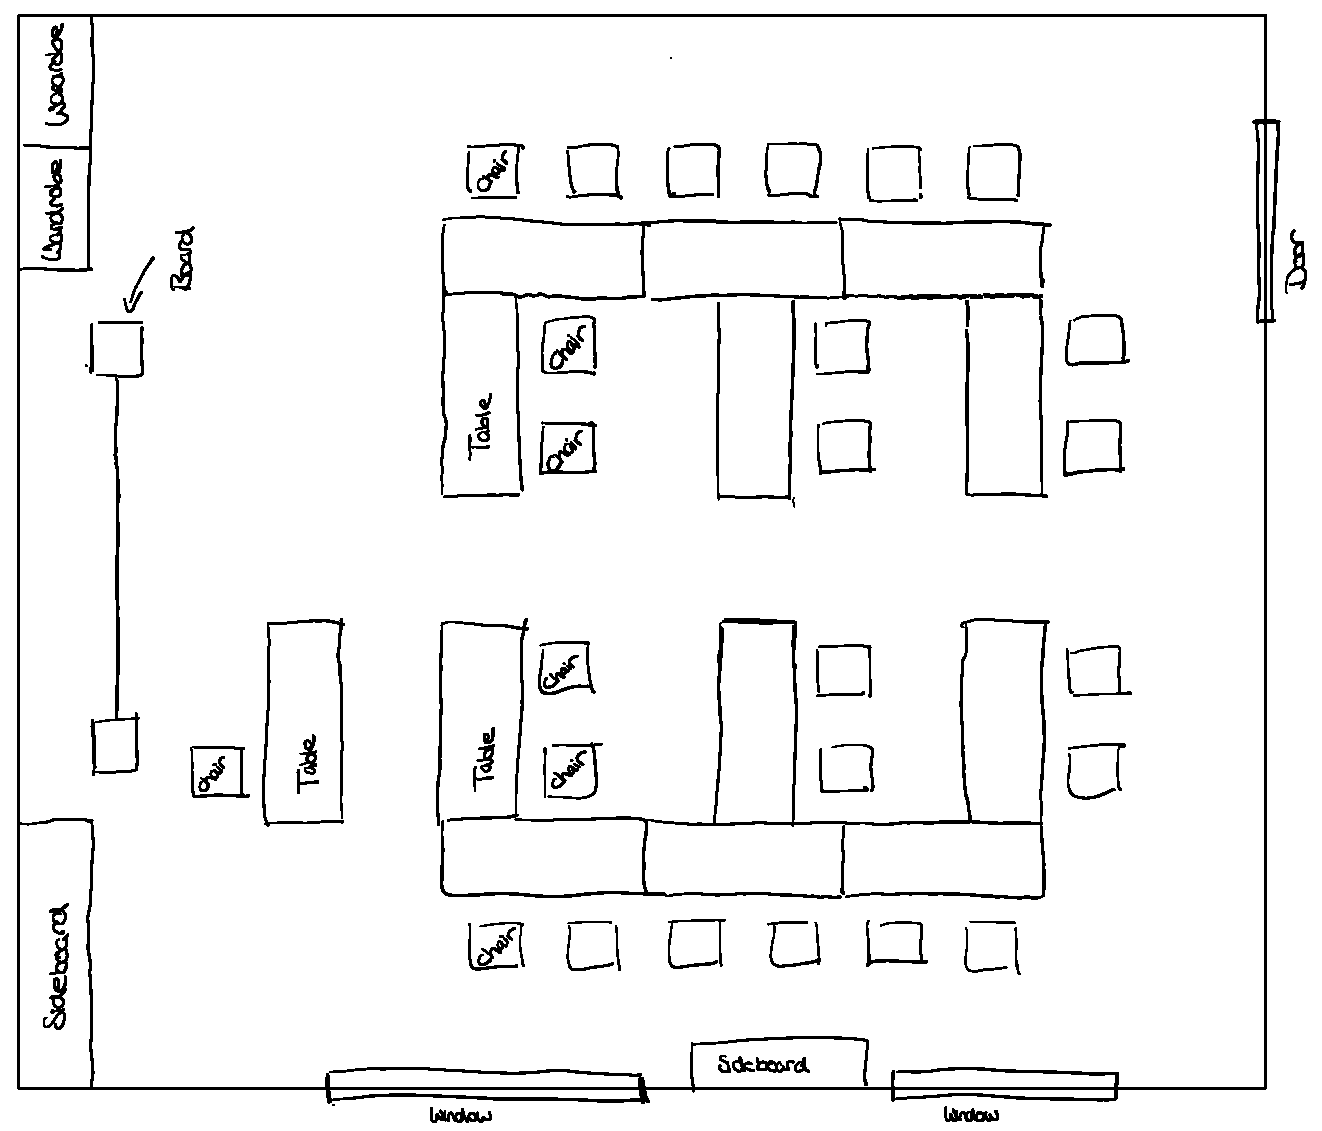
\includegraphics[width=1\textwidth]{images/roomModel_OneNote.pdf}
  \caption{Klassenzimmer Skizze}
  \label{fig:KlassenzimmerSkizze}
\end{figure}\noindent
Anschließend wurde der Raum maßstabsgetreu in einem Bauplan gezeichnet um so die Abstände und Maße teilweise zu definieren.
Diese Zeichnung ist in der Abbildung \ref{fig:KlassenzimmerEntwurf} dargestellt.

\begin{figure}[H]
  \centering
  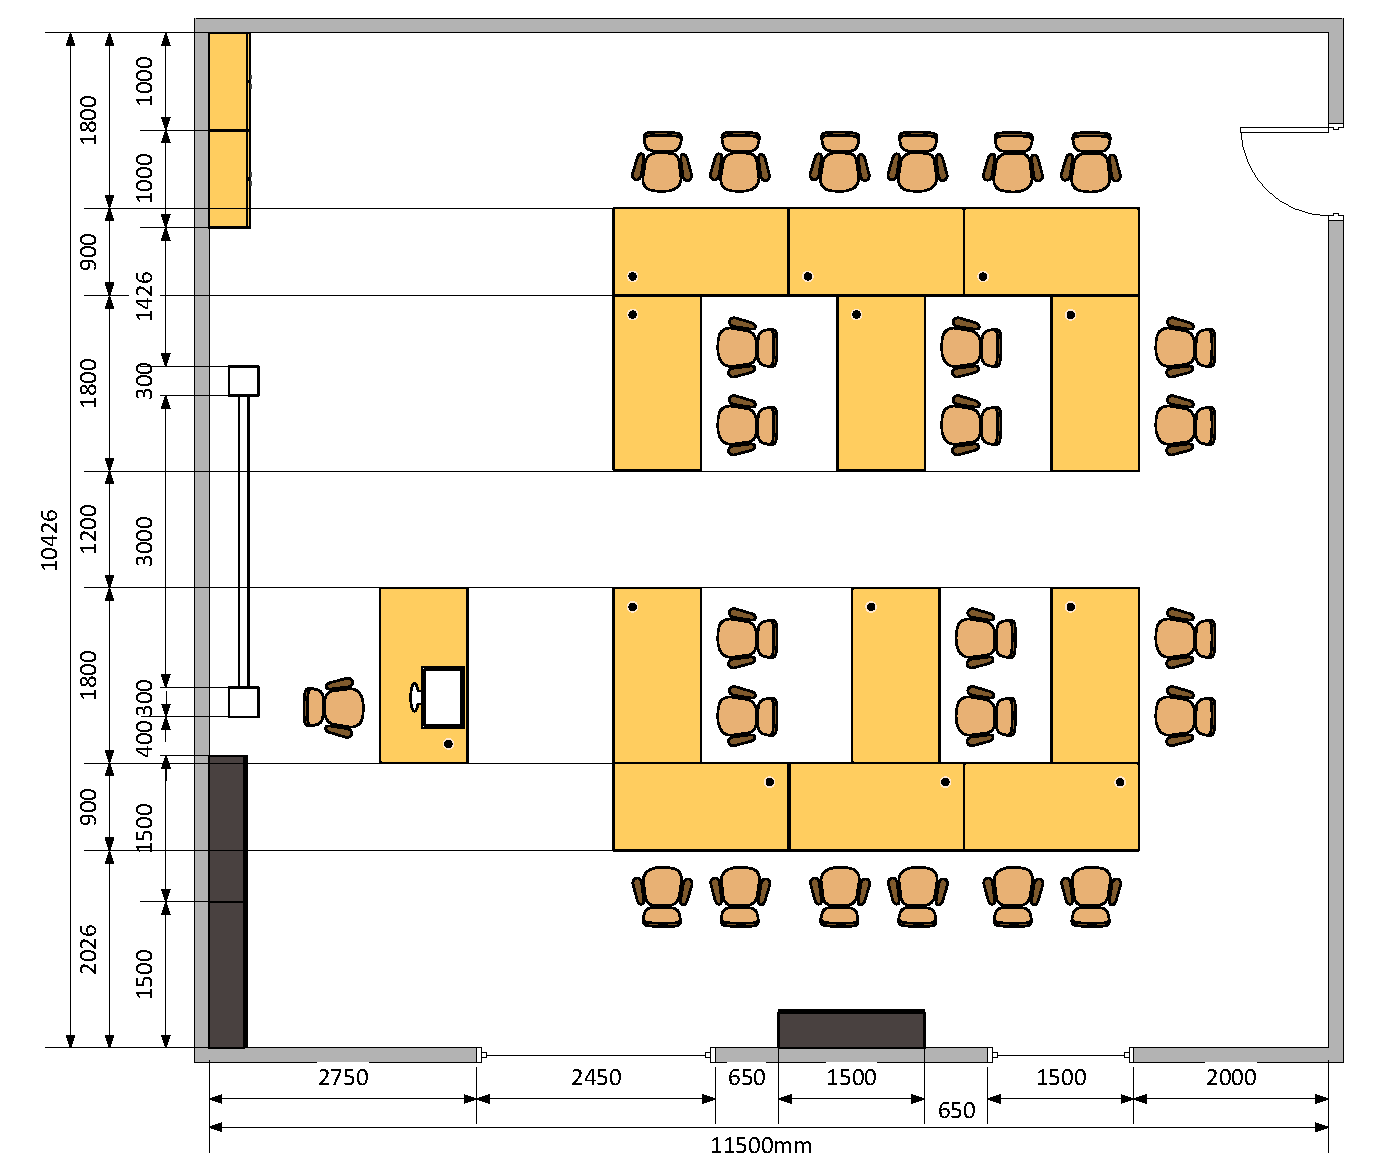
\includegraphics[width=1\textwidth]{images/classroom_draw.pdf}
  \caption{Klassenzimmer Entwurf mit Bemaßung}
  \label{fig:KlassenzimmerEntwurf}
\end{figure}\noindent
Um die Höhen der Fenster zu bestimmen wurde zusätzlich eine Seitenansicht erstellt.
Diese ist in der Abbildung \ref{fig:KlassenzimmerEntwurfWindows} zu sehen.
\begin{figure}[H]
  \centering
  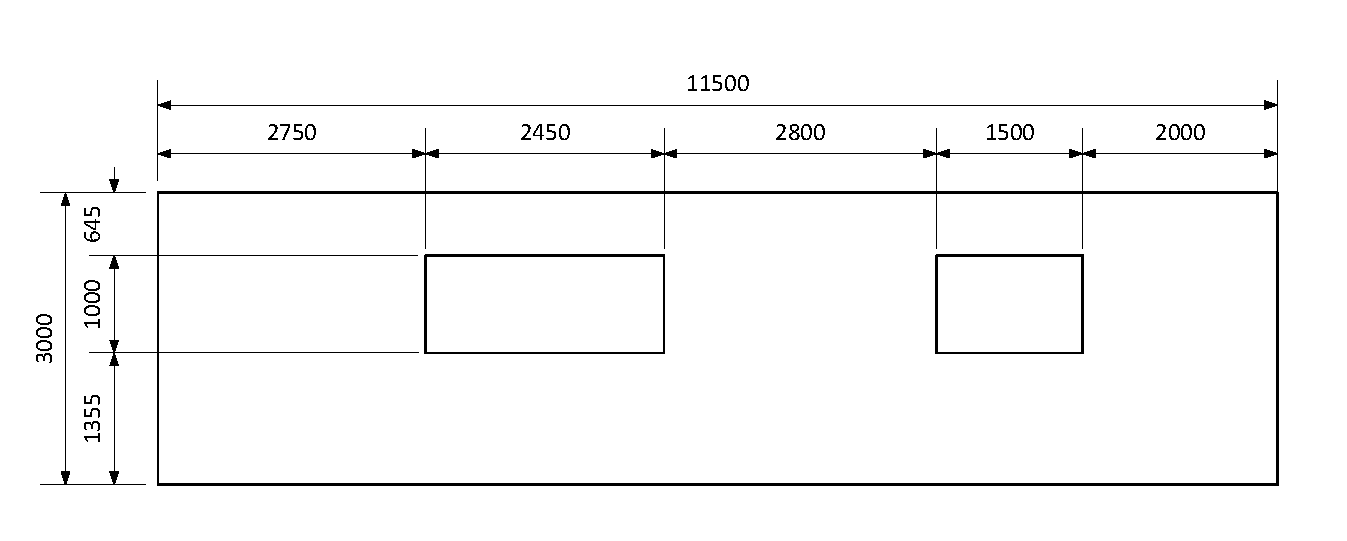
\includegraphics[width=1\textwidth]{images/classroom_draw_windows.pdf}
  \caption{Klassenzimmer Entwurf mit Fenster}
  \label{fig:KlassenzimmerEntwurfWindows}
\end{figure}\noindent
Abschließend wurde eine weitere Zeichnung zur Platzierung der Lampen erstellt. Diese ist in der Abbildung \ref{fig:KlassenzimmerEntwurfLamps}
dargestellt.
\begin{figure}[H]
  \centering
  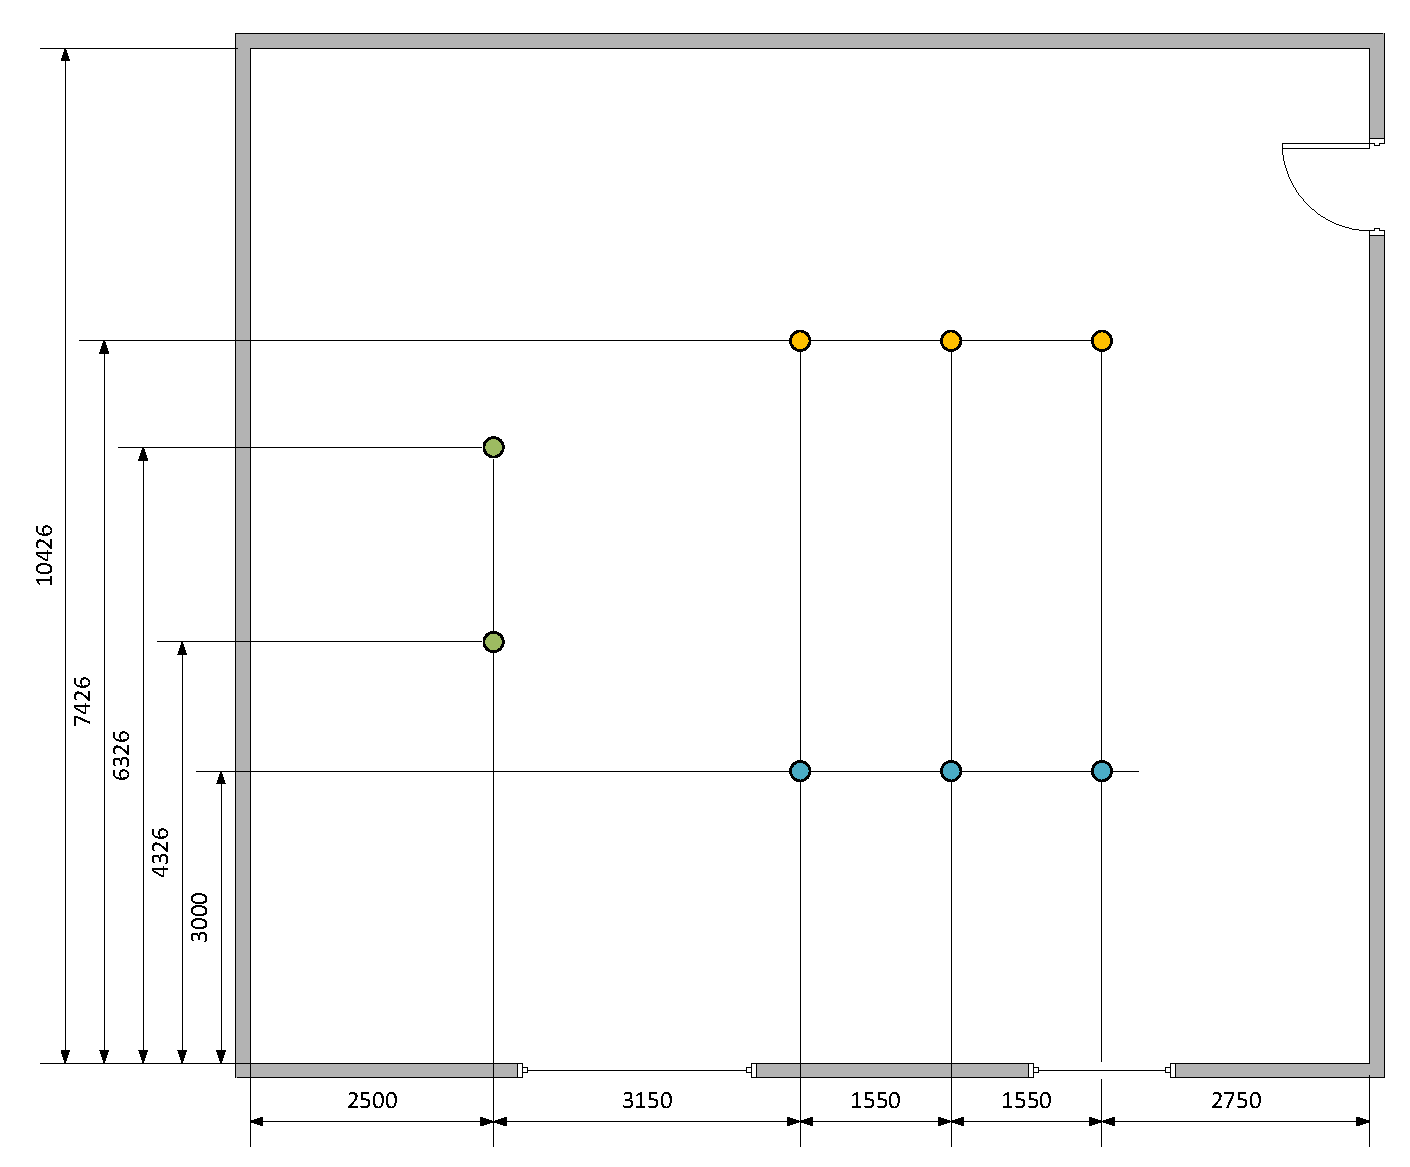
\includegraphics[width=1\textwidth]{images/classroom_draw_lamps.pdf}
  \caption{Klassenzimmer Entwurf der Lampen}
  \label{fig:KlassenzimmerEntwurfLamps}
\end{figure}\noindent
Um die Anforderungen vollständig zu erfüllen müssen Interaktionen mit der 3D Szene möglich sein, diese werden im Folgenden beschrieben.
\newparagraph
Im Klassenzimmer ist es möglich zu laufen, bei einer Kollision mit einem Gegenstand wird die Bewegung angehalten.
Das Licht im Klassenzimmer kann durch drei Lichtschalter neben der Tür per Mausklick gesteuert werden. Mit einem Schalter kann jeweils ein Cluster angesteuert werden, diese sind in Abb. \ref{fig:KlassenzimmerEntwurfLamps}
farblich gekennzeichnet.
% TODO: change! + HDR muss entfernt werden @Lukas?
Außerdem können die Stühle auf- und abgestuhlt werden. Bei einem Blick aus dem Fenster
soll die DHBW dargestellt werden, diese wird als \ac{HDR} Bild eingebunden. Zusätzlich können die Schränke geöffnet und geschlossen werden und die Tafel nach oben bzw. nach unten geschoben werden.
\newparagraph
Aus den beschrieben Animationen und den Plänen aus den Abbildung \ref{fig:KlassenzimmerEntwurf}, \ref{fig:KlassenzimmerEntwurfWindows} und \ref{fig:KlassenzimmerEntwurfLamps} ergeben sich alle Komponenten der Szene. 
Einige Maße werden bereits durch den Plan vorgegeben in einem weiteren Schritt werden diese nun vollständig definiert.
Diese Definition sind in der Tabelle \ref{tab:Komponenten} abgebildet.
\begin{table}[H]
  \centering
  \begin{tabular}{|l|c|c|c|c|}
    \hline
    \textbf{Komponente} & \textbf{x} & \textbf{y} & \textbf{z} & \textbf{file} \\
    \hline
    Blackboard & 03,600 & 00,240 & 02,500 & /blender/blackboard.glb \\
    \hline
    Chair & 00,470 & 00,480 & 00,870 & /blender/chair.glb \\
    \hline
    Closet & 01,000 & 00,725 & 02,200 & /blender/closet.glb \\
    \hline
    Lamp & 00,328 & 00,328 & 00,700 & /blender/lamp.glb \\
    \hline
    LightSwitch & 00,080 & 00,014 & 00,080 & /blender/lightswitch.glb \\
    \hline
    Sideboard & 00,600 & 01,500 & 00,700 & /blender/sideboard.glb \\
    \hline
    Table & 01,800 & 00,900 & 00,790 & /blender/table.glb \\
    \hline
    Room & 10,710 & 11,820 & 03,300 & /blender/room\_door.glb \\
    \hline
  \end{tabular}
  \caption{Modell-Maße in Meter}
  \label{tab:Komponenten}  
\end{table}
\noindent
Mit den definierten Größen aus Tabelle \ref{tab:Komponenten} können anschließend die Blender Modelle erstellt werden.
Um das Klassenzimmer ansprechender darzustellen werden weitere Elemente aus dem Internet eingefügt, diese werden mit ihren Quellen in Tabelle \ref{tab:KomponentenExtern} aufgezählt.
\begin{table}[H]
  \centering
  \begin{tabular}{|c|c|c|}
    \hline
    \textbf{Komponente} & \textbf{Quelle} & \textbf{file} \\
    \hline
    Monitor & https://poly.pizza/m/e8cELDeDuTr & /blender/monitor.glb \\
    \hline
    Keyboard & https://www.thingiverse.com/thing:4230507 & /blender/Keyboard.glb \\
    \hline
    \multirow{2}{*}{Plane}  & https://sketchfab.com/3d-models/low-poly-  & \multirow{2}{*}{/blender/basic\_plane.glb} \\ 
                            & airplane-65cc7c4349174f7bbb20ed70206377b5                                  & \\
    \hline
  \end{tabular}
  \caption{Modelle aus dem Internet}
  \label{tab:KomponentenExtern}
\end{table}
\subsection{Flugsimulator}
%johannes

Als Erweiterung der Flugschule, wird ein Flugsimulator-Spiel integriert, welches folgende Funktionen beinhaltet:
\newparagraph
Durch einen Klick auf den Monitor in der Flugschule wird auf eine Unterseite weitergeleitet und der Flugsimulator gestartet.
Ein Flugzeug-Modell wird in der Mitte der Szene platziert.
Dessen Flugrichtung ist mit der Maus veränderbar, wodurch eine Steuerung des Flugzeugs ermöglicht wird.
Die Geschwindigkeit des Flugzeugs wird nicht durch den Benutzer verändert, sondern passt sich anhand der Neigung des Flugzeugs an.
Mit einem Mausklick kann dem Flugzeug ein kleiner Boost gegeben werden.
\newparagraph
Beim Starten des Flugsimulator-Spiels wird ein Countdown gestartet, welcher 60 Sekunden lang dauert.
In dieser Zeit kann der Benutzer durch zufällig generierte Ringe fliegen und dabei (je nach Art des Rings) einen oder fünf Punkte sammeln.
Zur zusätzlichen Herausforderung werden Hindernisse generiert.
Wenn das Flugzeug in eines dieser Hindernisse oder gegen einen der Ringe fliegt oder die Zeit abläuft, wird das Spiel beendet.
Der Benutzer bekommt hierbei die erreichte Punktzahl angezeigt und kann das Spiel erneut starten oder zur Flugschule zurückkehren.
\newparagraph
Im Hindergrund des Spiels wird ein Ozean und ein Himmel dargestellt.
Die Kamera bewegt sich während des Fluges mit dem Flugzeug mit.
Die Steuerung kann durch das Drücken der Taste \texttt{I} invertiert werden, um allen Benutzern das bestmögliche Spielerlebnis zu ermöglichen.